\documentclass[aspectratio=169,10pt]{beamer}
\usetheme{Madrid}
\usecolortheme{seahorse}
\usepackage{amsmath,amssymb,amsthm}
\usepackage{xcolor}
\usepackage{listings}
\usepackage{graphicx}

\graphicspath{{figures/}}

\setbeamertemplate{footline}[frame number]
\setbeamertemplate{navigation symbols}{}

% Define colors
\definecolor{darkblue}{rgb}{0.1,0.2,0.5}
\definecolor{darkgreen}{rgb}{0.2,0.5,0.2}
\definecolor{darkred}{rgb}{0.7,0.0,0.0}

% Code listing setup
\lstset{
    basicstyle=\ttfamily\scriptsize,
    commentstyle=\color{darkgreen}\itshape,
    keywordstyle=\color{darkblue}\bfseries,
    stringstyle=\color{darkred},
    showstringspaces=false,
    breaklines=true,
    numbers=left,
    numberstyle=\tiny,
    frame=single,
    language=Python
}

\title[Chapter 6: Convex Cones]{Convex Cones and Generalized Interiors}
\subtitle{Bauschke \& Combettes, 2017 (Chapter 6)}
\author{Lecture on Convex Analysis}
\institute{Convex Analysis and Monotone Operator Theory}
\date{}

\begin{document}

% =============================================================================
% TITLE SLIDE
% =============================================================================
\begin{frame}
\titlepage
\end{frame}

% =============================================================================
% OUTLINE
% =============================================================================
\begin{frame}{Outline}
\tableofcontents
\end{frame}

% =============================================================================
% SECTION 6.1: CONVEX CONES
% =============================================================================
\section{6.1 Convex Cones}

\begin{frame}{What is a Convex Cone?}
\begin{definition}[Convex Cone]
A set $K \subseteq \mathcal{H}$ is a \textbf{cone} if
\[
(\forall \lambda \in \mathbb{R}_+) \quad \lambda K \subseteq K
\]
where $\mathbb{R}_+ = [0, \infty)$.
\end{definition}

\vspace{0.3cm}

\textbf{Interpretation:} If $x \in K$, then all positive scalar multiples $\lambda x$ are also in $K$.

\vspace{0.3cm}

\begin{proposition}[Properties of Cones]
\begin{itemize}
    \item A cone always contains the origin: $0 \in K$
    \item A cone closed under nonnegative combinations: if $x_i \in K$ and $\lambda_i \geq 0$, then $\sum_i \lambda_i x_i \in K$
    \item The intersection of cones is a cone
    \item The closure of a cone is a cone
\end{itemize}
\end{proposition}
\end{frame}

\begin{frame}{Example: The Positive Orthant}
\begin{example}[Positive Orthant]
The positive orthant in $\mathbb{R}^n$ is
\[
\mathbb{R}^n_+ = \{x = (x_1, \ldots, x_n) : x_i \geq 0 \text{ for all } i\}
\]
This is a closed, pointed, solid convex cone.
\end{example}

\vspace{0.3cm}

\begin{example}[Half-Space Cone]
Given $u \in \mathcal{H} \setminus \{0\}$, the set
\[
K = \{x \in \mathcal{H} : \langle x \mid u \rangle \leq 0\}
\]
is a solid convex cone, and it is not pointed if and only if $\dim \mathcal{H} > 1$.
\end{example}

\vspace{0.3cm}

\begin{figure}
    \centering
    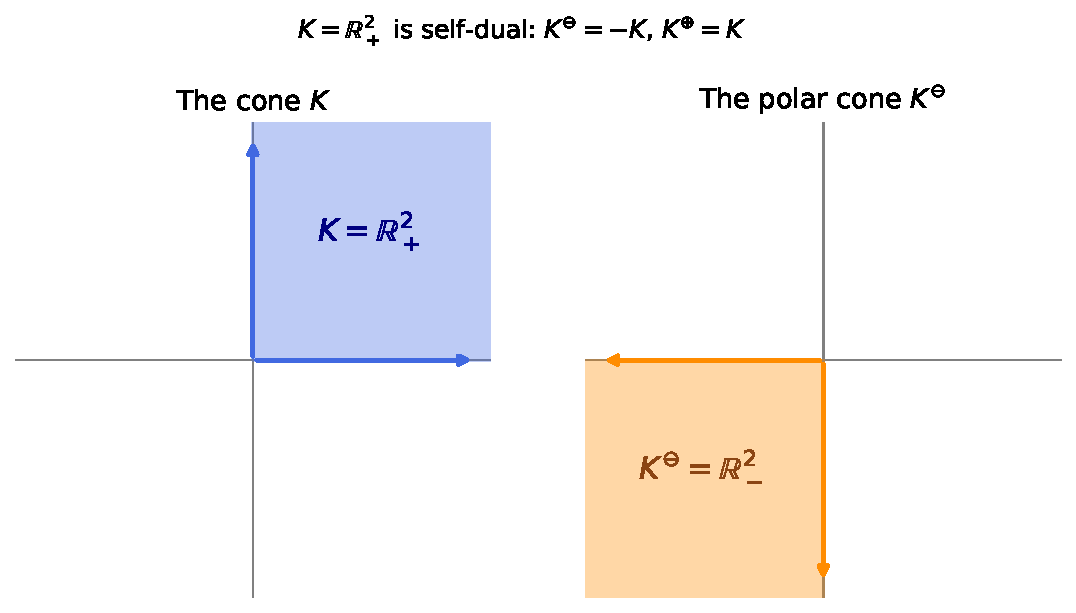
\includegraphics[width=0.5\textwidth]{fig_orthant_polar.pdf}
\end{figure}
\end{frame}

\begin{frame}{Cone Generated by a Set}
\begin{definition}
Given a set $C \subseteq \mathcal{H}$, the \textbf{cone} (or \textbf{conic hull}) generated by $C$ is
\[
\text{cone}(C) = \left\{\sum_{i \in I} \lambda_i x_i : I \text{ finite}, \lambda_i \in \mathbb{R}_+, x_i \in C\right\}
\]
\end{definition}

\vspace{0.3cm}

\begin{proposition}[6.2]
Let $D = \mathbb{R} \cdot C$. Then:
\begin{enumerate}
    \item $\text{cone}(C) \subseteq \text{cone}(D) = D$
    \item If $C$ is a cone, then $\text{cone}(C) = C$
    \item $\overline{\text{cone}(C)} = \text{cone}(\overline{C})$
\end{enumerate}
\end{proposition}

\vspace{0.3cm}

\begin{figure}
    \centering
    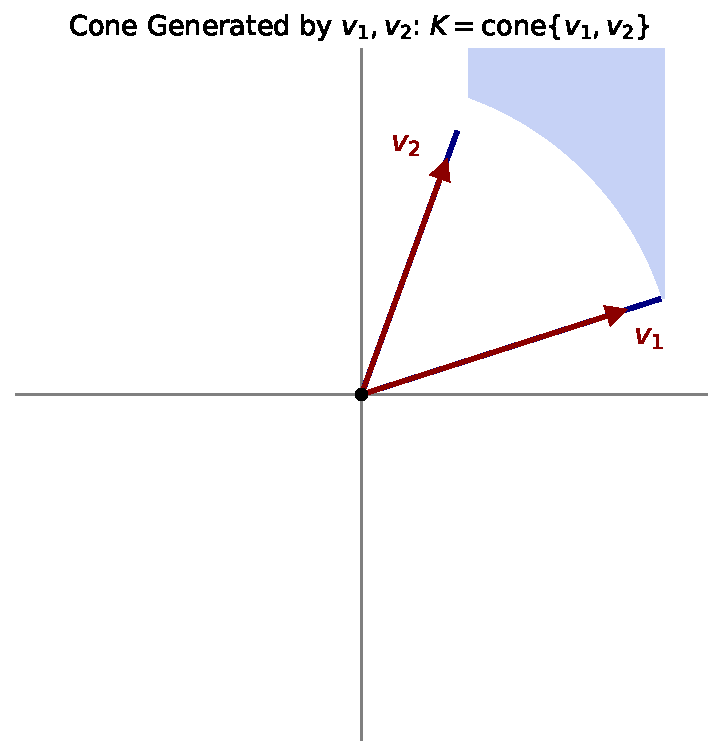
\includegraphics[width=0.6\textwidth]{fig_cone_generation.pdf}
\end{figure}
\end{frame}

\begin{frame}{Relationships Between Cones and Convex Sets}
\begin{proposition}[6.3]
Let $C$ be a subset of $\mathcal{H}$. Then:
\begin{itemize}
    \item[(i)] If $C$ is a cone, then $C$ is convex if and only if $C + C \subseteq C$.
    \item[(ii)] If $C$ is convex and $0 \in C$, then $C$ is a cone if and only if $C + C \subseteq C$.
\end{itemize}
\end{proposition}

\vspace{0.3cm}

\begin{proposition}[6.4]
Let $C$ be a nonempty convex subset of $\mathcal{H}$. Then:
\begin{itemize}
    \item[(i)] $\text{span}(C) = \text{cone}(C) - \text{cone}(C) = \text{cone}(C) + \text{cone}(-C)$
    \item[(ii)] If $C = -C$, then $\text{span}(C) = \text{cone}(C)$
\end{itemize}
\end{proposition}

\vspace{0.3cm}

\textbf{Key insight:} The cone generated by $C$ gives us the smallest cone containing $C$.
\end{frame}

\begin{frame}{Pointed and Solid Cones}
\begin{definition}[Pointed and Solid Cones]
Let $K$ be a convex cone in $\mathcal{H}$. Then:
\begin{itemize}
    \item $K$ is \textbf{pointed} if $K \cap (-K) \subseteq \{0\}$
    \item $K$ is \textbf{solid} if $\text{int}(K) \neq \emptyset$
\end{itemize}
\end{definition}

\vspace{0.3cm}

\begin{remark}
\begin{itemize}
    \item The only pointed linear subspace is $\{0\}$
    \item $\mathcal{H}$ is the only solid linear subspace
    \item The positive orthant $\mathbb{R}^n_+$ is both pointed and solid (for $n \geq 1$)
\end{itemize}
\end{remark}

\vspace{0.3cm}

\begin{example}[Half-Space]
The half-space $K = \{x \in \mathcal{H} : \langle x \mid u \rangle \leq 0\}$ is:
\begin{itemize}
    \item Solid (for any $u \neq 0$)
    \item Pointed if and only if $\dim \mathcal{H} = 1$
\end{itemize}
\end{example}

\begin{figure}
    \centering
    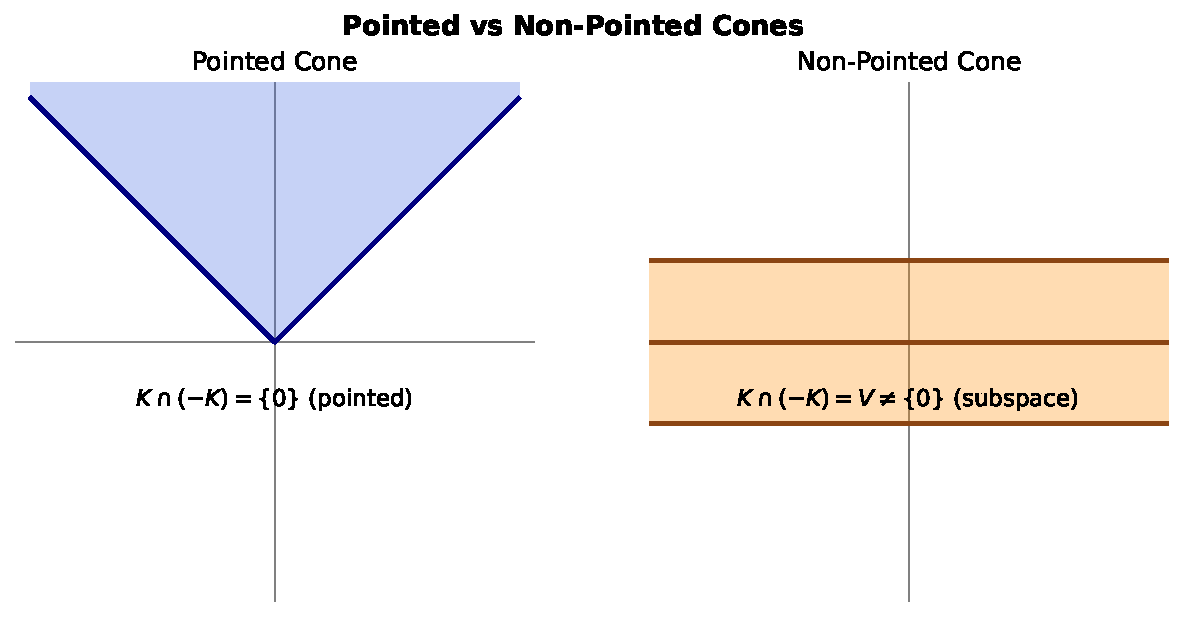
\includegraphics[width=0.6\textwidth]{fig_pointed_cones.pdf}
\end{figure}
\end{frame}

% =============================================================================
% SECTION 6.2: GENERALIZED INTERIORS
% =============================================================================
\section{6.2 Generalized Interiors}

\begin{frame}{Standard Interior}
Recall that the interior of a set $C$ is:
\[
\text{int}(C) = \{x \in C : (\exists \rho \in \mathbb{R}_{++}) B(\rho; x) \subseteq C - x\}
\]

\vspace{0.3cm}

For convex sets, we have the hierarchy:
\[
\text{int}(C) \subseteq \text{core}(C) \subseteq \text{sri}(C) \subseteq \text{ri}(C) \subseteq \text{qri}(C) \subseteq C
\]

\vspace{0.3cm}

\begin{definition}[Generalized Interiors]
Let $C$ be a convex subset of $\mathcal{H}$:
\begin{itemize}
    \item \textbf{Core:} $\text{core}(C) = \{x \in C : \text{cone}(C - x) = \mathcal{H}\}$
    \item \textbf{Strong relative interior:} $\text{sri}(C) = \{x \in C : \text{cone}(C - x) = \overline{\text{span}(C - x)}\}$
    \item \textbf{Relative interior:} $\text{ri}(C) = \{x \in C : \text{cone}(C - x) = \text{span}(C - x)\}$
    \item \textbf{Quasi-relative interior:} $\text{qri}(C) = \{x \in C : \overline{\text{cone}(C - x)} = \overline{\text{span}(C - x)}\}$
\end{itemize}
\end{definition}
\end{frame}

\begin{frame}{Key Properties of Generalized Interiors}
\begin{proposition}[6.10]
Let $C$ be a nonempty convex subset of $\mathcal{H}$ such that $C = -C$. Then:
\begin{itemize}
    \item[(i)] $0 \in \text{ri}(C)$
    \item[(ii)] If $\text{span}(C)$ is closed, then $0 \in \text{sri}(C)$
\end{itemize}
\end{proposition}

\vspace{0.3cm}

\begin{remark}
For any convex set $C$, we always have:
\[
\text{int}(C) \subseteq \text{core}(C) \subseteq \text{sri}(C) \subseteq \text{ri}(C) \subseteq \text{qri}(C) \subseteq C
\]
Each inclusion can be strict (see Example 6.11).
\end{remark}

\vspace{0.3cm}

\begin{figure}
    \centering
    \includegraphics[width=0.5\textwidth]{fig_core_relative_interior.pdf}
\end{figure}
\end{frame}

\begin{frame}[allowframebreaks]{Examples of Generalized Interiors}
\begin{example}[6.11]
\begin{itemize}
    \item[(i)] A proper closed linear subspace $V$ has $\text{core}(V) = \emptyset$ but $\text{sri}(V) = V$.

    \item[(ii)] In infinite-dimensional spaces, consider the set
    \[
    C = \left\{\sum_{n \in \mathbb{N}} \xi_n e_n : (\forall n) |\xi_n| \leq \frac{1}{4^n}\right\}
    \]
    Then $\text{cone}(C) \neq \overline{\text{span}(C)} = \mathcal{H}$, so $\text{core}(C) = \emptyset$.

    \item[(iii)] However, $0 \in \text{sri}(C)$ (with stronger growth condition) when the span is closed.
\end{itemize}
\end{example}

\framebreak

\begin{key_observation}
The key difference between $\text{ri}(C)$ and $\text{core}(C)$ is whether we require the closure:
\begin{align*}
x \in \text{core}(C) &\Rightarrow \text{cone}(C - x) = \mathcal{H} \\
x \in \text{sri}(C) &\Rightarrow \text{cone}(C - x) = \overline{\text{span}(C - x)}
\end{align*}

In infinite dimensions, this distinction matters significantly!
\end{key_observation}
\end{frame}

% =============================================================================
% SECTION 6.3: POLAR AND DUAL CONES
% =============================================================================
\section{6.3 Polar and Dual Cones}

\begin{frame}{Polar and Dual Cones}
\begin{definition}[Polar Cone]
Given a set $K$ in $\mathcal{H}$, the \textbf{polar cone} is
\[
K^{\ominus} = \{u \in \mathcal{H} : (\forall x \in K) \langle u \mid x \rangle \leq 0\}
\]
\end{definition}

\vspace{0.3cm}

\begin{definition}[Dual Cone]
The \textbf{dual cone} is
\[
K^{\oplus} = \{u \in \mathcal{H} : (\forall x \in K) \langle u \mid x \rangle \geq 0\} = -K^{\ominus}
\]
\end{definition}

\vspace{0.3cm}

\textbf{Relationship:} $K^{\oplus} = -K^{\ominus}$ (the dual cone is the negative polar).

\vspace{0.3cm}

\begin{key_observation}
\begin{itemize}
    \item If $K$ is a cone, then $K^{\ominus}$ and $K^{\oplus}$ are both closed convex cones
    \item $(K^{\ominus})^{\ominus} = \overline{\text{cone}(K)}$ (bipolar theorem)
    \item $\mathbb{R}^n_+$ is self-dual: $(\mathbb{R}^n_+)^{\oplus} = \mathbb{R}^n_+$
\end{itemize}
\end{key_observation}

\begin{figure}
    \centering
    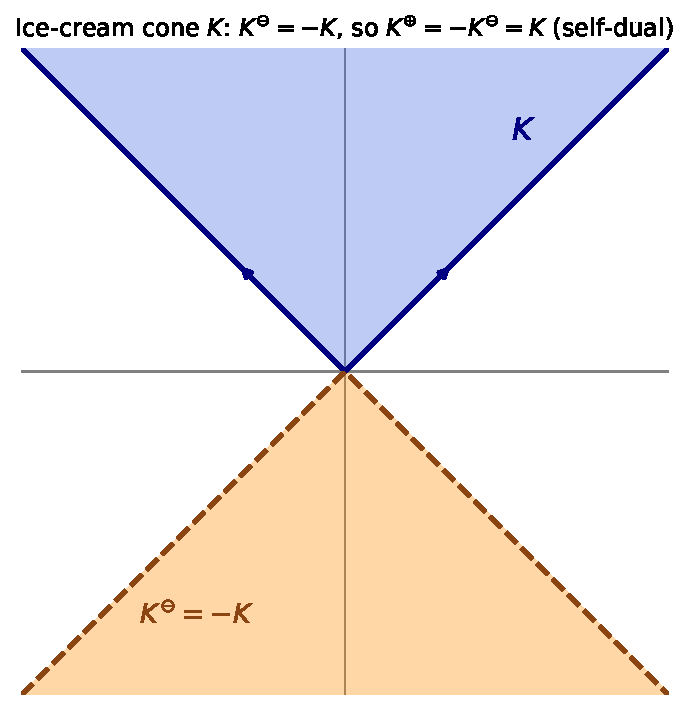
\includegraphics[width=0.5\textwidth]{fig_icecream_dual.pdf}
\end{figure}
\end{frame}

\begin{frame}{Properties of Polar and Dual Cones}
\begin{proposition}[6.24]
Let $K$ be a nonempty closed convex cone in $\mathcal{H}$, let $x \in \mathcal{H}$, and let $p \in \mathcal{H}$.
Then
\[
p = P_K x \Leftrightarrow [p \in K, \, x - p \in K^{\oplus}]
\]

\vspace{0.3cm}

Equivalently,
\[
p = P_K x \Leftrightarrow [p \in K, \, x - p \in K^{\ominus}]
\]
\end{proposition}

\vspace{0.3cm}

\textbf{Interpretation:} The projection onto $K$ is characterized using the dual cone.

\vspace{0.3cm}

\begin{theorem}[6.30 - Moreau]
Let $K$ be a nonempty closed convex cone in $\mathcal{H}$ and let $x \in \mathcal{H}$. Then:
\begin{enumerate}
    \item $x = P_K x + P_{K^{\oplus}} x$
    \item $P_K x \perp P_{K^{\oplus}} x$
    \item $\|x\|^2 = d_K^2(x) + d_{K^{\oplus}}^2(x)$
\end{enumerate}
\end{theorem}
\end{frame}

\begin{frame}{Self-Dual Cones}
\begin{definition}
A cone $K$ is \textbf{self-dual} if $K^{\oplus} = K$ (or equivalently, $K^{\ominus} = -K$).
\end{definition}

\vspace{0.3cm}

\begin{example}
\begin{itemize}
    \item The positive orthant $\mathbb{R}^n_+$ is self-dual
    \item The ice-cream (second-order) cone $\{(x,y) \in \mathbb{R}^{n-1} \times \mathbb{R} : y \geq \|x\|\}$ is self-dual
    \item The Lorentz cone is self-dual
\end{itemize}
\end{example}

\vspace{0.3cm}

\begin{figure}
    \centering
    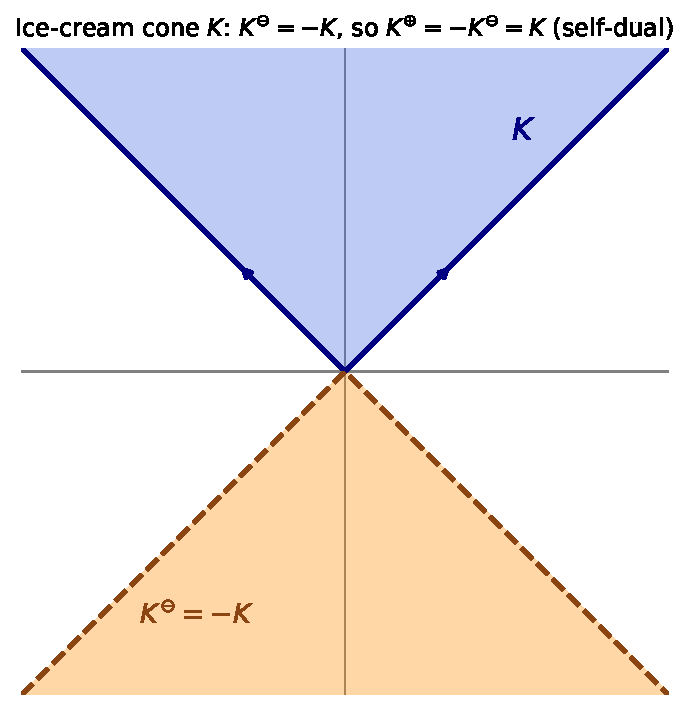
\includegraphics[width=0.7\textwidth]{fig_icecream_dual.pdf}
\end{figure}
\end{frame}

\begin{frame}{Projection onto Cones}
\begin{proposition}[6.28]
Let $K$ be a nonempty closed convex cone in $\mathcal{H}$, let $x \in \mathcal{H}$, and let $p \in \mathcal{H}$.
Then $p = P_K x$ if and only if
\[
p \in K, \quad x - p \in K^{\ominus}, \quad \langle x - p \mid p \rangle = 0
\]
\end{proposition}

\vspace{0.3cm}

\textbf{Key property:} The orthogonality condition $\langle x - p \mid p \rangle = 0$ is crucial.

\vspace{0.3cm}

\begin{example}[6.29]
Let $\mathcal{H} = \ell^2(I)$, $K = \ell^2_+(I)$, and $x = (\xi_i)_{i \in I}$. Then
\[
P_K x = (\max\{\xi_i, 0\})_{i \in I}
\]
This is the componentwise positive part operation.
\end{example}
\end{frame}

% =============================================================================
% SECTION 6.4: TANGENT AND NORMAL CONES
% =============================================================================
\section{6.4 Tangent and Normal Cones}

\begin{frame}{Tangent Cone}
\begin{definition}[Tangent Cone]
Let $C$ be a nonempty convex subset of $\mathcal{H}$ and let $x \in \mathcal{H}$. The \textbf{tangent cone} to $C$ at $x$ is
\[
T_C x = \begin{cases}
\overline{\text{cone}(C - x)} = \bigcup_{\lambda \in \mathbb{R}_{++}} \lambda(C - x) & \text{if } x \in C; \\
\emptyset & \text{otherwise}
\end{cases}
\]
\end{definition}

\vspace{0.3cm}

\begin{remark}
\begin{itemize}
    \item If $x \in C$, then $T_C x$ is a nonempty closed convex cone containing $0$
    \item At an interior point: $T_C x = \mathcal{H}$
    \item At a boundary point, $T_C x$ captures directions we can move into $C$
\end{itemize}
\end{remark}

\vspace{0.3cm}

\begin{figure}
    \centering
    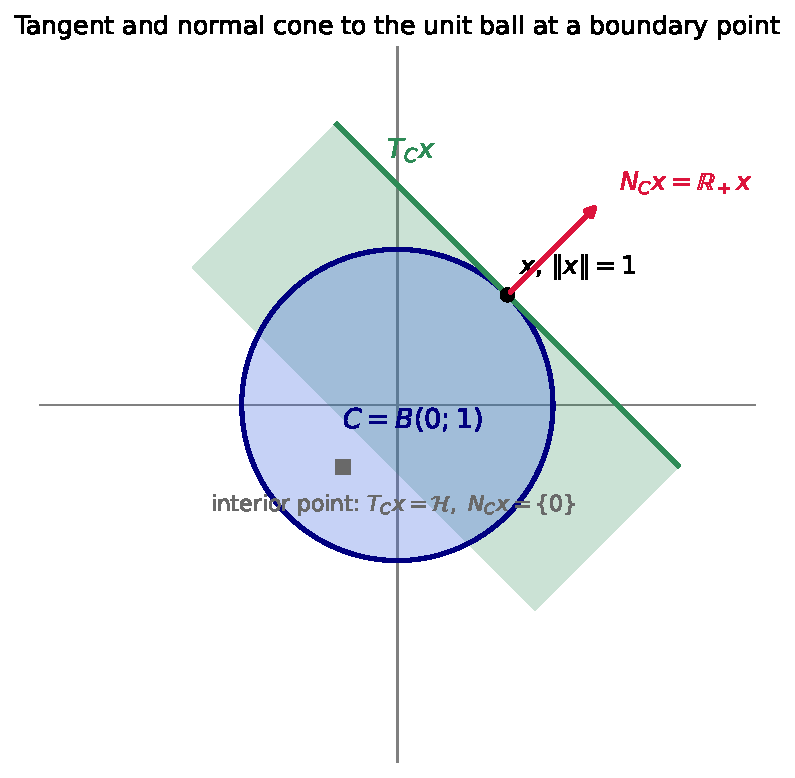
\includegraphics[width=0.6\textwidth]{fig_ball_tangent_normal.pdf}
\end{figure}
\end{frame}

\begin{frame}{Normal Cone}
\begin{definition}[Normal Cone]
Let $C$ be a nonempty convex subset of $\mathcal{H}$ and let $x \in \mathcal{H}$. The \textbf{normal cone} to $C$ at $x$ is
\[
N_C x = \{u \in \mathcal{H} : (\forall y \in C) \langle u \mid y - x \rangle \leq 0\}
\]
\end{definition}

\vspace{0.3cm}

\textbf{Interpretation:} $u \in N_C x$ means $u$ points ``outward'' from the tangent directions.

\vspace{0.3cm}

\begin{key_observation}
\begin{itemize}
    \item If $x \notin C$, then $N_C x = \emptyset$ (definition extends to: $N_C x = \emptyset$ if $x \notin C$, or alternatively, $N_C x = \{u : \text{the hyperplane } \{y : \langle u \mid y - x \rangle = 0\} \text{ supports } C\}$)
    \item If $x \in C$, then $N_C x$ is a nonempty closed convex cone
    \item At an interior point: $N_C x = \{0\}$
\end{itemize}
\end{key_observation}

\begin{figure}
    \centering
    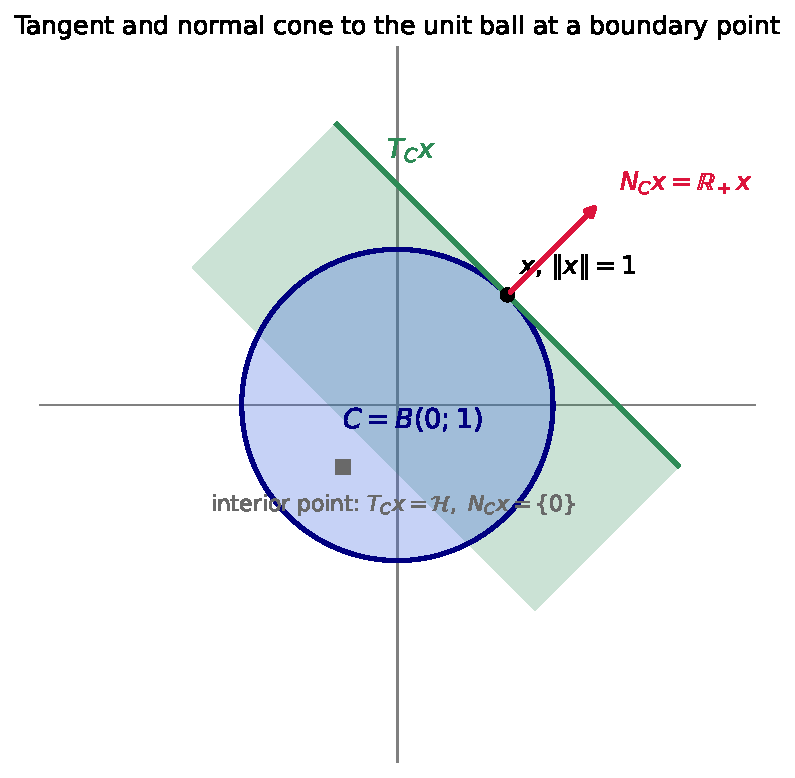
\includegraphics[width=0.5\textwidth]{fig_ball_tangent_normal.pdf}
\end{figure}
\end{frame}

\begin{frame}{Relationship Between Tangent and Normal Cones}
\begin{proposition}[6.44]
Let $C$ be a nonempty convex subset of $\mathcal{H}$ and let $x \in C$. Then:
\begin{enumerate}
    \item $T_C^{\oplus} x = N_C x$ and $N_C^{\oplus} x = T_C x$
    \item If $x \in \text{core}(C)$, then $T_C x = \mathcal{H} \Leftrightarrow N_C x = \{0\}$
\end{enumerate}
\end{proposition}

\vspace{0.3cm}

\begin{proposition}[6.45]
Let $C$ be a convex subset of $\mathcal{H}$ such that $\text{int}(C) \neq \emptyset$ and let $x \in C$. Then:
\[
x \in \text{int}(C) \Leftrightarrow T_C x = \mathcal{H} \Leftrightarrow N_C x = \{0\}
\]
\end{proposition}

\vspace{0.3cm}

\textbf{Key insight:} The tangent and normal cones are orthogonal complements!
\end{frame}

\begin{frame}{Examples of Tangent and Normal Cones}
\begin{example}[6.39 - Unit Ball]
For $C = B(0; 1) = \{x \in \mathcal{H} : \|x\| \leq 1\}$ and $x \in C$ with $\|x\| = 1$:
\[
T_C x = \{y \in \mathcal{H} : \langle y \mid x \rangle \leq 0\}, \quad N_C x = \mathbb{R}_+ x
\]
\end{example}

\vspace{0.3cm}

\begin{example}[6.40 - Ice-Cream Cone]
For the ice-cream cone $K = \{(x,y) \in \mathbb{R}^{n-1} \times \mathbb{R} : y \geq \|x\|\}$ at $x_0 = (x_0, y_0)$ with $y_0 > \|x_0\|$:
\[
T_K x_0 = \{(x, y) : y \geq \|x\|\}, \quad N_K x_0 = \mathbb{R}_+ \cdot \frac{(x_0, -\|x_0\|)}{\sqrt{2\|x_0\|^2 + 1}}
\]
\end{example}

\vspace{0.3cm}

\begin{figure}
    \centering
    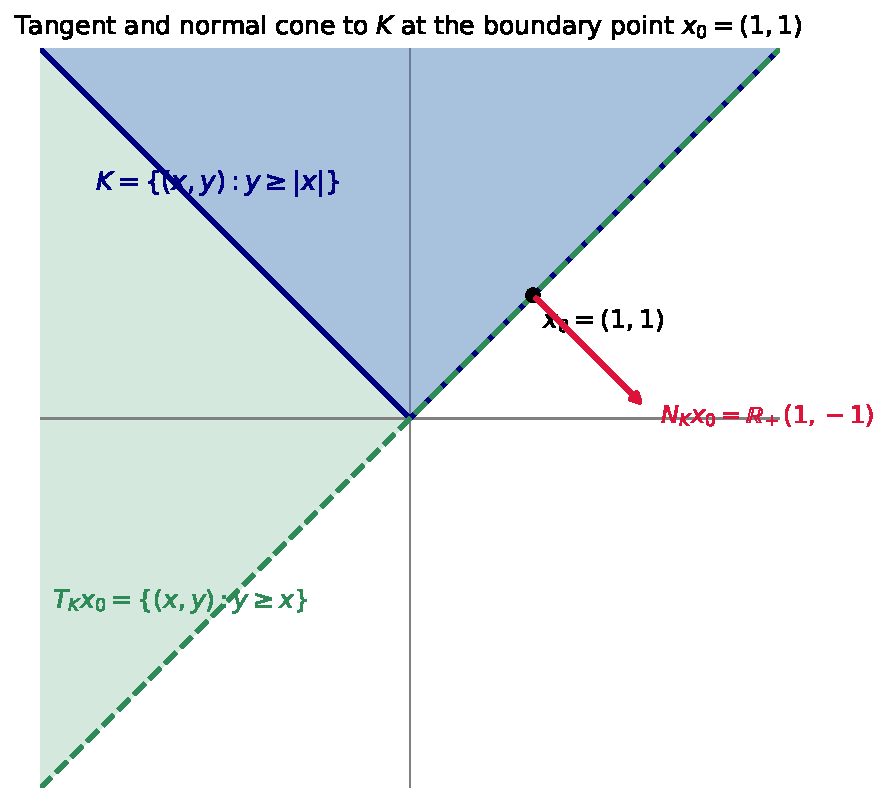
\includegraphics[width=0.6\textwidth]{fig_cone_tangent_normal.pdf}
\end{figure}
\end{frame}

\begin{frame}{Characterization of Interior Points}
\begin{corollary}[6.46]
Suppose that $\mathcal{H}$ is finite-dimensional, let $C$ be a nonempty convex subset of $\mathcal{H}$, and let $x \in C$. Then the following are equivalent:
\begin{enumerate}
    \item $x \in \text{int}(C)$
    \item $T_C x = \mathcal{H}$
    \item $N_C x = \{0\}$
\end{enumerate}
\end{corollary}

\vspace{0.3cm}

\begin{proposition}[6.47]
Let $C$ be a nonempty closed convex subset of $\mathcal{H}$, and let $x$ and $p$ be points in $\mathcal{H}$.
Then $p = P_C x$ if and only if $x - p \in N_C p$.
\end{proposition}

\vspace{0.3cm}

\textbf{Key insight:} The projection characterization uses the normal cone in a fundamental way.
\end{frame}

% =============================================================================
% NUMERICAL EXAMPLES AND PYTHON CODE
% =============================================================================
\section{Numerical Examples}

\begin{frame}[fragile]{Python Example: Projection onto Positive Orthant}
\begin{lstlisting}
import numpy as np

def project_onto_positive_orthant(x):
    """
    Project a vector x onto the positive orthant R_+^n.

    For convex cones: P_K(x) = (max(x_i, 0))_{i=1}^n
    """
    return np.maximum(x, 0)

# Example
x = np.array([2, -1, 3, -0.5, 1])
proj_x = project_onto_positive_orthant(x)
print(f"Original: {x}")
print(f"Projection onto R_+^n: {proj_x}")

# Verify: x - proj_x should be in K^* = {u: <u,y> >= 0 for y in K}
residual = x - proj_x  # [-2, -1, 0, -0.5, 0] (all <= 0 dual cone)
print(f"Residual: {residual}")
\end{lstlisting}

\vspace{0.3cm}

\textbf{Output:}
\begin{itemize}
    \item Original: [2, -1, 3, -0.5, 1]
    \item Projection: [2, 0, 3, 0, 1]
    \item Residual: [0, -1, 0, -0.5, 0] (in dual cone)
\end{itemize}
\end{frame}

\begin{frame}[fragile]{Python Example: Polar Cone}
\begin{lstlisting}
import numpy as np

def check_in_polar_cone(x, u):
    """
    Check if u is in the polar cone K^- = {u: <u,x> <= 0 for all x in K}
    For K = R_+^n, this is R_-^n (the negative orthant).
    """
    return np.dot(u, x) <= 1e-10  # numerical tolerance

# Example: K = R_+^2
K_x = np.array([1, 2])  # in K = R_+^2

u1 = np.array([-1, -1])   # in K^- (polar)
u2 = np.array([1, 1])     # NOT in K^-

print(f"x = {K_x} in K = R_+^2")
print(f"u1 = {u1}: <u1, x> = {np.dot(u1, K_x)} <= 0? {check_in_polar_cone(K_x, u1)}")
print(f"u2 = {u2}: <u2, x> = {np.dot(u2, K_x)} <= 0? {check_in_polar_cone(K_x, u2)}")

# Verify: K^- = -K (self-dual property of R_+^n)
print(f"\nFor K = R_+^n: K^- = -K (self-dual)")
\end{lstlisting}

\vspace{0.3cm}

\textbf{Output:}
\begin{itemize}
    \item u1 = [-1, -1]: <u1, x> = -3 <= 0? True
    \item u2 = [1, 1]: <u2, x> = 3 <= 0? False
\end{itemize}
\end{frame}

\begin{frame}[fragile]{Python Example: Tangent and Normal Cones}
\begin{lstlisting}
import numpy as np

def tangent_cone_ball(x, radius=1.0):
    """
    For C = B(0, r), at point x with ||x|| <= r:
    T_C(x) = {y : <y | x> <= 0} if ||x|| = r (boundary)
             H if ||x|| < r (interior)
    """
    norm_x = np.linalg.norm(x)
    if np.isclose(norm_x, radius):
        return "T_C(x) = {y : <y | x> <= 0}"  # half-space
    else:
        return "T_C(x) = H (entire space)"

def normal_cone_ball(x, radius=1.0):
    """
    For C = B(0, r), at point x with ||x|| <= r:
    N_C(x) = R_+ * x if ||x|| = r (boundary)
             {0} if ||x|| < r (interior)
    """
    norm_x = np.linalg.norm(x)
    if np.isclose(norm_x, radius):
        return f"N_C(x) = R_+ * {x/norm_x}"  # ray
    else:
        return "N_C(x) = {0}"

# Example on unit ball boundary
x_boundary = np.array([1.0, 0.0])  # ||x|| = 1
x_interior = np.array([0.5, 0.5])   # ||x|| = sqrt(0.5) < 1

print("Unit ball C = B(0, 1):")
print(f"At boundary point x = {x_boundary}:")
print(f"  {tangent_cone_ball(x_boundary)}")
print(f"  {normal_cone_ball(x_boundary)}")
print(f"\nAt interior point x = {x_interior}:")
print(f"  {tangent_cone_ball(x_interior)}")
print(f"  {normal_cone_ball(x_interior)}")
\end{lstlisting}
\end{frame}

% =============================================================================
% KEY THEOREMS AND RESULTS
% =============================================================================
\section{Key Theorems and Results}

\begin{frame}{Fundamental Decomposition}
\begin{theorem}[Projection Decomposition]
Let $K$ be a nonempty closed convex cone. Then for every $x \in \mathcal{H}$:
\[
x = P_K x + P_{K^{\oplus}} x
\]
with
\[
P_K x \perp P_{K^{\oplus}} x \quad \text{and} \quad \|x\|^2 = \|P_K x\|^2 + \|P_{K^{\oplus}} x\|^2
\]
\end{theorem}

\vspace{0.3cm}

\textbf{Interpretation:} Every vector can be uniquely decomposed into a component in the cone and one in the dual cone, with orthogonality.

\vspace{0.3cm}

\begin{corollary}[6.31]
Let $K$ be a nonempty closed convex cone in $\mathcal{H}$, and let $x \in \mathcal{H}$.
Suppose that $y \in K$ and $z \in K^{\oplus} \setminus \{P_{K^{\oplus}} x\}$ satisfy $x = y + z$. Then:
\begin{enumerate}
    \item $\|P_K x\| \leq \|y\|$ and $\|P_{K^{\oplus}} x\| \leq \|z\|$
    \item $\langle y \mid z \rangle = \langle P_K x \mid P_{K^{\oplus}} x \rangle = 0$
    \item $\|P_K x - P_{K^{\oplus}} x\| < \|y - z\|$
\end{enumerate}
\end{corollary}
\end{frame}

\begin{frame}{Summary of Key Properties}
\begin{center}
\begin{tabular}{|l|c|c|}
\hline
\textbf{Property} & \textbf{Cone $K$} & \textbf{Dual/Polar} \\
\hline
Nonempty & Yes & Yes \\
Closed & Yes & Yes \\
Convex & Yes & Yes \\
Contains 0 & Yes & Yes \\
\hline
\textbf{Self-Duality} & \multicolumn{2}{c|}{$K^{\oplus} = K$ for some cones} \\
\hline
\textbf{Bipolar} & \multicolumn{2}{c|}{$(K^{\ominus})^{\ominus} = \overline{\text{cone}(K)}$} \\
\hline
\end{tabular}
\end{center}

\vspace{0.5cm}

\begin{itemize}
    \item \textbf{Positive Orthant:} Pointed, solid, self-dual
    \item \textbf{Half-space:} Solid, not pointed (unless dim = 1)
    \item \textbf{Linear subspace:} Both a cone and its own polar (up to sign)
    \item \textbf{Ice-cream cone:} Pointed, solid, self-dual
\end{itemize}
\end{frame}

\begin{frame}[allowframebreaks]{Applications and Connections}
\begin{itemize}
    \item \textbf{Optimization:} Convex cones appear naturally in conic programming
    \begin{itemize}
        \item Linear conic programs: minimize $\langle c \mid x \rangle$ subject to $Ax \in K$
        \item KKT conditions involve normal cones
    \end{itemize}

    \item \textbf{Duality:} Lagrange multipliers lie in the dual cone
    \begin{itemize}
        \item Primal: minimize $f(x)$ subject to $x \in K$
        \item Dual involves $K^{\oplus}$
    \end{itemize}

    \item \textbf{Monotone Operator Theory:} Normal cones define subdifferentials
    \begin{itemize}
        \item Subdifferential $\partial f(x) = N_{\text{epi}(f)}(x, f(x))$
        \item Used in proximal algorithms
    \end{itemize}

    \item \textbf{Matrix Optimization:} Semidefinite cones $\mathbb{S}^n_+$
    \begin{itemize}
        \item Convex cones in the space of symmetric matrices
        \item Self-dual: $(\mathbb{S}^n_+)^{\oplus} = \mathbb{S}^n_+$
    \end{itemize}
\end{itemize}
\end{frame}

% =============================================================================
% CONCLUSION
% =============================================================================
\begin{frame}{Summary}
\begin{enumerate}
    \item \textbf{Convex Cones:} Fundamental objects containing $0$ and closed under positive scaling

    \item \textbf{Generalized Interiors:} Multiple notions adapted for non-Euclidean spaces (core, sri, ri, qri)

    \item \textbf{Polar \& Dual Cones:} Orthogonal complements in the cone setting; crucial for optimization

    \item \textbf{Tangent \& Normal Cones:} Characterize boundary behavior; dual pairs via polarity

    \item \textbf{Key Result:} Projection decomposition $x = P_K x + P_{K^{\oplus}} x$ with orthogonality
\end{enumerate}

\vspace{0.5cm}

\textbf{Next Chapter:} Support functions and polar sets generalize these ideas further.
\end{frame}

\begin{frame}{References}
\begin{itemize}
    \item \textbf{Bauschke, H. H., \& Combettes, P. L.} (2017).
    \textit{Convex Analysis and Monotone Operator Theory in Hilbert Spaces}.
    Springer, 2nd edition. Chapter 6.

    \item \textbf{Boyd, S., \& Vandenberghe, L.} (2004).
    \textit{Convex Optimization}. Cambridge University Press.
    (Chapters on convex sets and cones)

    \item \textbf{Rockafellar, R. T.} (1970).
    \textit{Convex Analysis}. Princeton University Press.
    (Classic reference on convex analysis)
\end{itemize}

\vspace{0.5cm}

\centerline{\Large Thank you!}
\end{frame}

\end{document}
